\chapter{System Design and Architecture}
\label{ch:system-design}
\quad In this chapter, there is a full description of each module design and architecture in our project. First, an overview and any needed assumptions we used will be explained. Then the overall system architecture and block diagram. Then for each module, there is a functional description, modular decomposition, design constraints, and any other needed descriptions. In addition to the decisions, we took about the modules' functionalities. \\

During the development and implementation of our project, we made sure the project code is modular and clear enough to be understood, in case of any future need for the code itself.

\bigskip
\noindent 
The overall system could be broken down to mainly 4 components:
\begin{itemize}[itemsep=1pt, topsep=5pt]
    \item \textbf{Page segmentation}: \\Computer vision techniques to prepare unseen handwritten image pages to be extracted into lines and words.
    \item \textbf{Model development}:\\ End-to-end deep learning network used to predict and recognize unseen segmented manuscript images.
    \item \textbf{Applications development}:\\ Web and mobile applications developed and integrated with deep learning networks as user-friendly services. 
    \item \textbf{Testing}:\\ Set of scripts, programs, and \acrfull{gui} for system testing and development. 
\end{itemize}

This chapter discusses the first 2 modules, while the applications development and testing are discussed in chapters \ref{ch:system-development} and \ref{ch:system-testing}, because it's not part of the final deployed system, but rather built for testing and development purposes.

\clearpage

\section{Overview and Assumptions}
\acrshort{asar} project consists of 3 main modules that need to be completely understood before starting implementing such a thing. These three are line segmentation, word segmentation, and pattern recognition. Apart from that, there is the connection between each module and the other, the research and modularity that needs to be considered. Each of these modules is described in detail in the following section, and how they all connect to each other, and how they represent the system architecture. \\

\noindent
Some assumptions are also considered in delivering this project are: 
\subsection{Accuracy}
Since the Arabic language has difficult problems to deal with such as styling format that is different from writer to writer, and from age to age.
We will use the hybrid technology to introduce a good accuracy in recognizing Arabic words or characters in whatever style are writing.

\subsection{Speed}
The system will try to recognize the manuscript documents have a lot of lines and words in a reasonable time. 

\subsection{Friendly Interface}
The system is developed into two (web and mobile) applications with a friendly interface that gives the user the accessibility to have an account, upload, crop, and download the document results.

\section{System Architecture}
% The aronal fieldchitecture of your system should be given in this section. This architecture should be first represented as a block diagram (subsection 5.2.1), which clarifies different project modules and the connections between them. You may add more subsections to properly explain your design. If possible, flowcharts are better included to ensure that the big picture and the interaction between different modules are very clear to the reader. Thereafter, each module should have a separate subsequent section to clearly describe and discuss it.

The system's main modules can be explained in this flow:
\begin{itemize}[itemsep=1pt, topsep=5pt]
    \item Image Preprocessing
    \item Page Segmentation
    \begin{itemize} 
        \item Line Segmentation
        \item Word Segmentation
    \end{itemize}
    \item Word Spotting
    \item Model Development
\end{itemize}

\noindent
In image preprocessing, we will prepare the manuscript image to be passed into the next module by applying some morphological operations such as normalization, adaptive thresholding, and median subtraction. After the image is preprocessed, we will extract each line segment by using the contours of the image, then we will take the largest contours area as segmented lines. The output of these lines will go into some another morphological operations to extract each word in this which has the lowest histogram to separate between words. \\

\noindent
After each word is extracted from the manuscript image, it will be embedded into the trained model to analyze and predict the corresponding transcript. Model development, image preprocessing, line, and word segmentation are explained in detail in the following subsections.

\section{Block Diagram}

\begin{figure}[!htb]
    \centering
    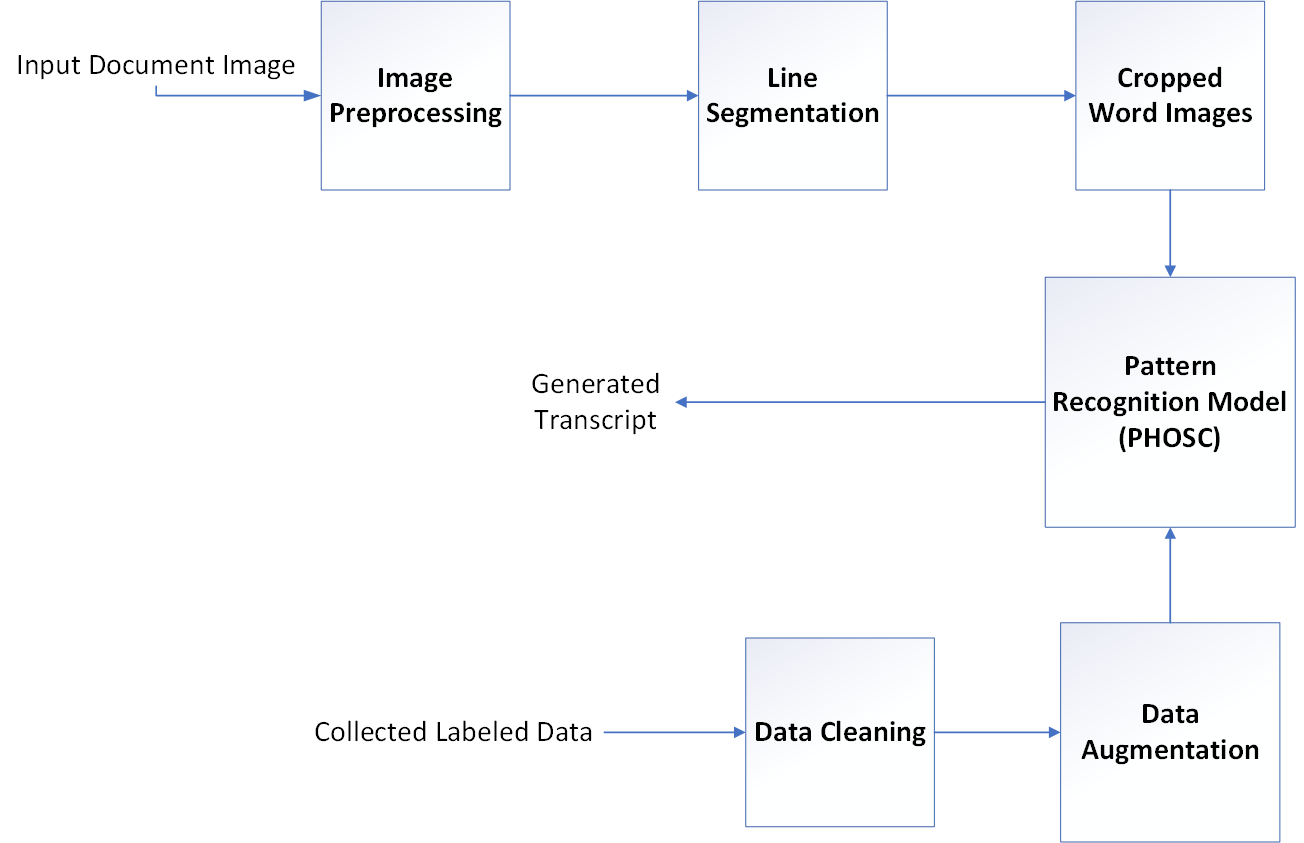
\includegraphics[width=12cm]{images/block diagram.png}
    \caption{ASAR Architecture Block Diagram}
    \label{fig:block-digram}
\end{figure}

\section{Image Preprocessing}
This module is responsible for preprocessing techniques that are used in document images as an initial step in the segmentation system. Most of preprocessing techniques are application-specific and not all preprocessing techniques have to be applied to all applications. Each application may require different preprocessing techniques depending on the different factors that may affect the quality of its images, such as those we applied to images for segmentation.

\subsection{Functional Description}
Preprocessing is the preliminary step that transforms the data into a format that will be more easily and effectively processed. Therefore, the main task in preprocessing the captured data is to decrease the variation that causes a reduction in the efficiency  rate and increases the complexities, for example, preprocessing of the input raw stroke of characters is crucial for the success of efficient character recognition systems. Thus, preprocessing is an essential stage prior to controlling the suitability of the results for the successive stages. 


\subsection{Modular Decomposition}
Image enhancement improves the quality of images for human perception by removing noise, reducing blurring, increasing contrast, and providing more detail \cite{inbook}. 

\begin{itemize}[labelindent=1em,labelsep=0.25cm,leftmargin=*]
        \item[\char `A)] \textbf{Resize Image:-}\\
        Images are normalized into a specific size, decided empirically or experimentally depending on the application and the feature extraction or classification techniques used, then features are extracted from all images  with the same size in order to provide data uniformity. 
        \item[\char `B)] \textbf{Normalization:-}\\  
        The Histogram Equalization \cite{equalization} evenly distributes the occurrence of pixel intensities so that the entire range of intensities is considered. This method usually increases the global contrast of images, especially when the usable data of the image is represented by close contrast values. Through this adjustment, the intensities can be better distributed on the histogram. This allows for areas of lower local contrast to gain a higher contrast. Histogram equalization accomplishes this by effectively spreading out the most frequent intensity values. Then probability density function (pdf) is calculated for the histogram shown Figure\ref{fig:equalize}.
        \begin{figure}[!htb]
            \centering
            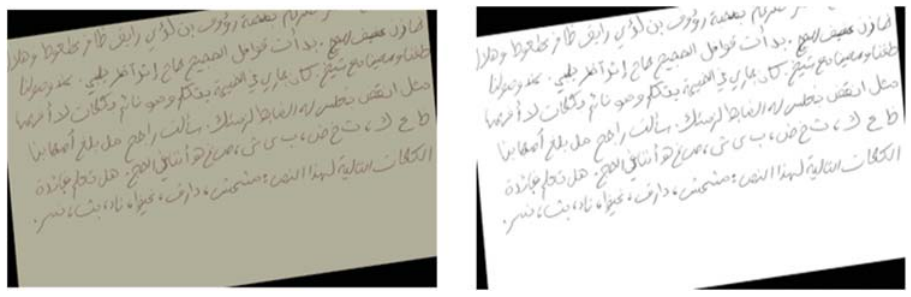
\includegraphics[width=11cm]{images/equalize.png}
            \caption{Affective result of proposed adaptive histogram equalization}
            \label{fig:equalize}
        \end{figure}
        \item[\char `C)] \textbf{Gaussian Blur:-}\\ 
        applying a Gaussian filter of a standard deviation   $\sigma$ for noise
        reduction purposes, the gradient magnitude is then computed using the
        simple energy function:
        
        \begin{equation}
            e(I) = [\frac{\partial}{\partial x} I] + [\frac{\partial}{\partial y} I]
            \label{equ:blur}
        \end{equation}
        \item[\char `D)] \textbf{Gray Scaling:-}\\
        A grayscale (or graylevel) image is simply one in which the only colors are shades of gray. The reason for differentiating such images from any other sort of color image is that less information needs to be provided for each pixel.so, it is only necessary to specify a single intensity value for each pixel, as opposed to the three intensities needed to specify each pixel in a full-color image.
        grayscale images are entirely sufficient for an easy process and so there is no need to use more complicated and harder-to-process color images.
        
        the input RGB fundus image $(I)$ is converted to a grayscale image ($Ig$) using Eq.\ref{equ:gray}.
        
        \begin{equation}
            Ig = 0.2989 * IR + 0.5870 * IG + 0.1140 * IB
            \label{equ:gray}
        \end{equation}
        \item[\char `E)] \textbf{Gaussian Thresholding (OTSU):-}\\
        The goal of thresholding \cite{thresholding} an image is to classify pixels as either “dark” or “light”.\\
        There are numerous methods for image thresholding which already been used by some researchers. The most common thresholding method has been proposed by Otsu . Otsu’s method works better where the clear separation between foreground and background exists or where image illumination is not variable shown in figure \ref{fig:otsu}. However, real-life images possess especially in handwriting images various kinds of degradations (e.g. illumination contrast, skewed, stains, and noise) that weaken the thresholding proposed by Otsu’s. Gaussian thresholding (OTSU) with binary inverse shown in figure\ref{fig:otsubnv}.
        \begin{figure}[!htb]
            \centering
            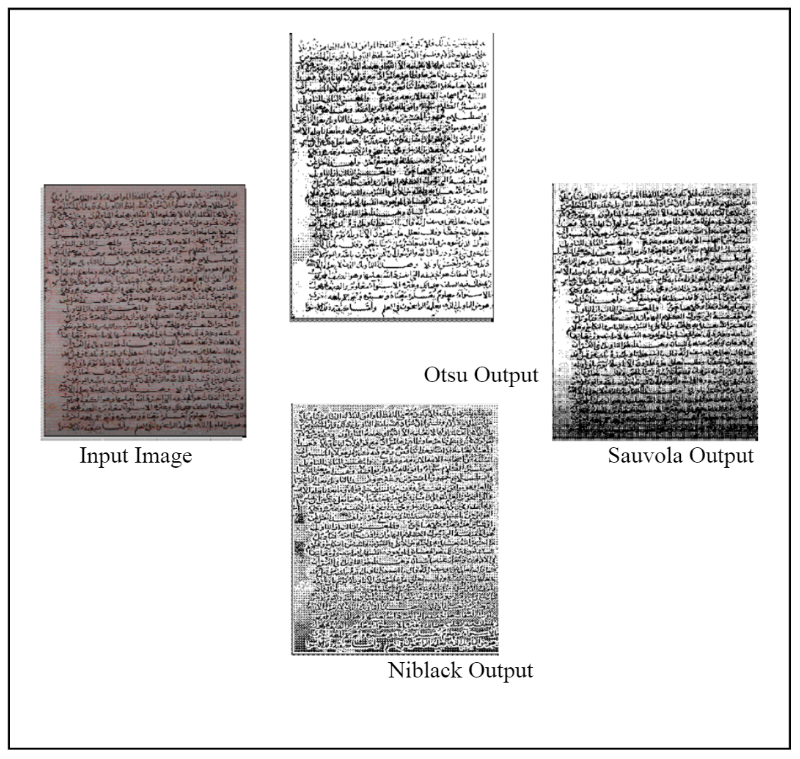
\includegraphics[width=11cm]{images/otsu.png}
            \caption{Images results of various thresholding methods}
            \label{fig:otsu}
        \end{figure}
        
        \begin{figure}[H]
            \centering
            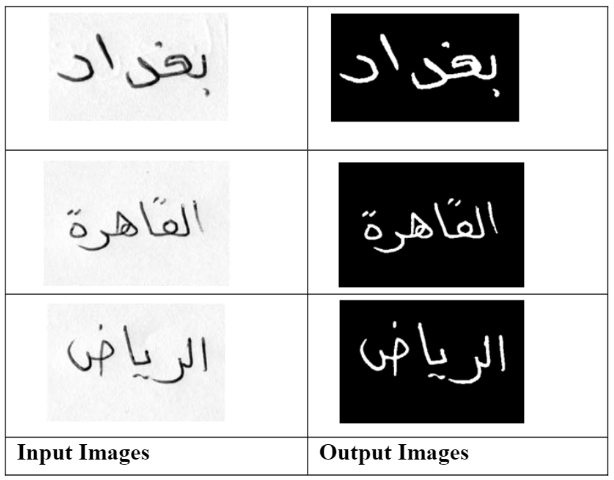
\includegraphics[width=7cm]{images/otsu-binv.png}
            \caption{Gaussian thresholding (OTSU) with binary inverse}
            \label{fig:otsubnv}
        \end{figure}
         \item[\char `F)] \textbf{Median Subtraction:-}\\
         Removing noise is to remove information coming from the
        background such as show-through effects, interfering strokes
        due to the seeping of ink during a long period of storage, spots of
        humidity and curvature effect. Example for the image before
        using the filter method shown in figure\ref{fig:bfmed} 
        
        \begin{figure}[!htb]
            \centering
            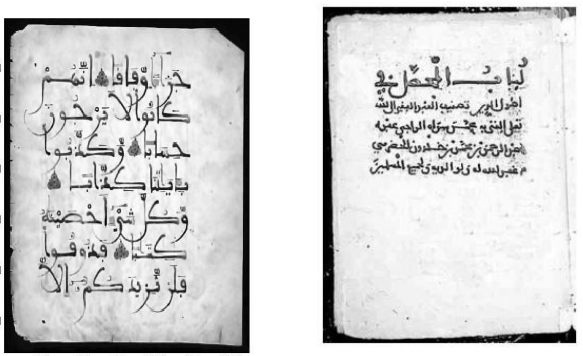
\includegraphics[width=9cm]{images/bmedian.png}
            \caption{Before using filter}
            \label{fig:bfmed}
        \end{figure}
        
        In median filtering \cite{median}, the neighboring pixels are ranked
        according to brightness (intensity) and the median value
        becomes the new value for the central pixel, shown in figure\ref{fig:afmed}.
        the value of an output pixel is determined by the median of the
        neighborhood pixels.
        
        \begin{figure}[!htb]
            \centering
            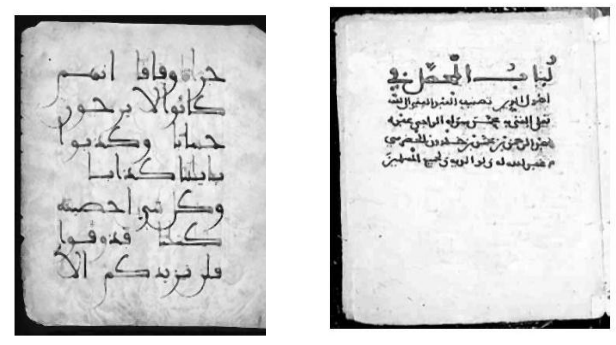
\includegraphics[width=9cm]{images/afmedian.png}
            \caption{Using median filter}
            \label{fig:afmed}
        \end{figure}
    \end{itemize}

\section{Line Segmentation}
This module is responsible for applying the text-line segmentation technique. Text-line segmentation is recognized as being an important step for handwritten text recognition because inaccurate segmentation will cause errors in the recognition step. %..

\subsection{Functional Description}
In this module, we will apply our method for text-line segmentation. Figure \ref{fig:flow_line} shows the flowchart of the proposed system. The proposed method consists of two stages. In the first stage, the mathematical morphology technique is used for constructing bridges between the components. In the next stage, find contours technique is proposed for the segmentation of the text into lines.
        \begin{figure}[!htb]
            \centering
            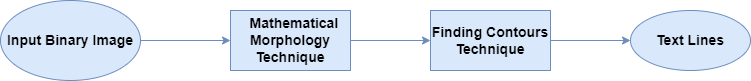
\includegraphics[width=14cm]{images/flowchart_line_segmentation.png}
            \caption{Flowchart of the proposed line segmentation method. }
            \label{fig:flow_line}
        \end{figure}
\subsection{Modular Decomposition}
This module could be separated into two distinct sub-modules depending on each other, and we will discuss them in detail. %..

\subsubsection{Morphology}
Mathematical morphology is a tool for extracting image components that are useful in the representation and description of region shapes, such as boundaries, skeletons, and the convex hull. Dilation is a primitive morphological operation that grows or thickens objects in a binary image. The specific manner and extent of this thickening is controlled by a shape referred to as a structuring element. Structuring elements are small sets or sub-images used to probe an image under study for properties of interest.

There are two basic morphological operators: erosion and dilation. These operators are usually applied in tandem. Opening and closing are two derived operations defined in terms of erosion and dilation.

\begin{itemize}
        \item {\textbf{Erosion:}}\\
            The erosion operation uses a structuring
            element for reducing or shrinking the shapes contained in the input image:
        
            \begin{equation}
                 A \ominus B = \left\{Z |  B_{z} \subset A \right\}
                \label{equ:Erosion-function}
                \end{equation}
            where A is the image, B is the structure element, and z is the points in B.
                
    \item {\textbf{Dilation:}}\\
            The dilation operation uses a structuring element characteristics for expanding the image:
        
            \begin{equation}
                A \oplus  B = \left\{Z |  B_{z} \bigcap  A \neq \phi  \right\}
                \label{equ:Dilation-function}
            \end{equation}
            where A is the image, B is the structure element, and z is the points in B.
            \item {\textbf{Opening:}}\\
            The opening is defined as an erosion followed by a dilation using the same structuring element. Opening of a grey-level image A and structuring element B, denoted \textbf{A $\circ $ B} , is defined as follows:
        \begin{equation}
            A \circ  B = \left ( A \ominus B \right ) \oplus B
            \label{equ:Opening-function}
        \end{equation}
            
            \item {\textbf{Closing:}}\\
            Closing is defined as a dilation followed by an erosion using the same structuring element for both operations. Closing of a grey-level image A and structuring element B, denoted \textbf{A $\bullet$ B} , is defined as follows:
        \begin{equation}
            A \bullet B = \left ( A \oplus   B \right ) \ominus B
            \label{equ:Clocing-function}
        \end{equation}
            
    \end{itemize}
\noindent
As it can be seen above and in general in any morphological operation the structuring element used to probe the input image, is the most important part.

\noindent
A structuring element is a matrix consisting of only 0's and 1's that can have any arbitrary shape and size. Typically are much smaller than the image being processed, while the pixels with values of 1 define the neighborhood. The center pixel of the structuring element, called the origin, identifies the pixel of interest – the pixel being processed.
\noindent
For example, Figure\ref{fig:structuring-element} illustrates a diamond-shaped structuring element of 7x7 size.
\begin{figure}[!htb]
    \centering
    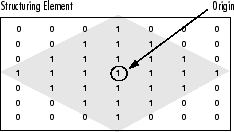
\includegraphics[width=5cm]{images/SE.png}
    \caption{A Diamond-Shaped Structuring Element and its Origin}
    \label{fig:structuring-element}
\end{figure} \\


To begin with, a set of sequential morphological operators is applied to the binary image figure \ref{fig:input_binary_img} to extract points that have high gradients to their background as the contrast feature and to obtain a processed image version, with the intention that every connected pixel component represents a text line.Figure \ref{fig:Flowchart_MO} shows the whole procedure of our novel morphology-based technique to extract the feature. The series of morphological operations will be discussed in the following:%Done
\begin{figure}[H]
    \centering
    
\includegraphics[width=6cm, height=9cm]{images/input.png}
    \caption{Binary Images that are the input to morphological operations}
    \label{fig:input_binary_img}
\end{figure}

\begin{itemize}
        \item[\char `a)] \textbf{Closing:-}
         
         A closing is used to close holes inside of objects or for connecting components together.Figure \ref{fig:closing} shows the result after applying the closing on the binary input  image.
         
         The closing operation has filled in gaps that are smaller than or the same size as the structuring element. Hence, the closing could be useful for connecting objects that are near each other, while not affecting objects that are too far apart.

        \begin{figure}[!htb]
             \centering
             \begin{subfigure}[b]{0.4\textwidth}
                 \centering
                 
\includegraphics[width=6cm, height=9cm]{images/clos1.png}
                 \caption{closing: [20,5]}
                 \label{fig:close1}
             \end{subfigure}
             \hfill
             \begin{subfigure}[b]{0.4\textwidth}
                 \centering
                 
\includegraphics[width=6cm, height=9cm]{images/clos2.png}
                 \caption{closing: [35,1]}
                 \label{fig:close2}
             \end{subfigure}
            \caption{Applying a morphological closing operation to our input image.}
            \label{fig:closing}
        \end{figure}

        \item[\char `b)] \textbf{Erosion:-}
        
        We have used morphological operations, mainly, erosion to extract the useful foreground and background information. Erosion is one of two fundamental operations in morphological image processing from which all other morphological operations are based. For details about this see \cite{esosion}. After Closing, we will have a smoothed image, where the foreground part belongs to black text regions and the background part consists of white regions. By erosion, we determine some important information from the foreground and background portions which are very helpful in our line segmentation purpose.
        
        Figure \ref{fig:erosio_img} shows the result after applying the erosion to our image after the closing step.

        \item[\char `c)] \textbf{Blurring:-}\\
        When we blur an image, we make the color transition from one side of an edge in the image to another smooth rather than sudden. So, we’ll do is apply an average blur on the image after erosion  using a 99 x 1 kernel. This will help smooth out high-frequency noise in our image. A blur is a very common operation we need to perform before other tasks such as thresholding.
        
        This figure \ref{fig:Blurring} shows this operation.
        
         \begin{figure}[!htb]
             \centering
             \begin{subfigure}[b]{0.4\textwidth}
                \centering
                
\includegraphics[width=6cm, height=9cm]{images/erosion.png}
                \caption{Applying erosion to our image}
                \label{fig:erosio_img}
             \end{subfigure}
             \hfill
             \begin{subfigure}[b]{0.4\textwidth}
                \centering
                
\includegraphics[width=6cm, height=9cm]{images/blureImg.png}
                \caption{Blurring to our image}
                \label{fig:Blurring}
             \end{subfigure}
            \caption{The sample after applying erosion and blurring}
            \label{fig:erosion-blurring}
        \end{figure}
        
        \newpage
        
        \item[\char `d)] \textbf{Thresholding:-}\\
        The thresholding is a key step in our segmentation method, its aim is to threshold the resulting smoothed image in order to isolate the blobs corresponding to line components.
        
        Now, we can apply Simple Thresholding to Blurred images as shown in figure \ref{fig:treshold_img}.
        
        \begin{figure}[H]
            \centering
            
\includegraphics[width=6cm, height=9cm]{images/threthold.png}
            \caption{Applying simple thresholding.}
            \label{fig:treshold_img}
        \end{figure}
        
        \newpage

        \item[\char `e)] \textbf{Dilation}\\
        Finally, We applied the dilation operation on the Thresholding image to make objects more visible and fill in small holes in objects. Lines appear thicker, and filled shapes appear larger. Dilation makes the groups of text to be detected more accurately as shown in the figure \ref{fig:Dilation_img}.%Done
        
        \item[\char `f)] \textbf{Labeling}\\
        This step aims to show all connected regions in the dilated image by applying connected-component labeling as shown in the figure \ref{fig:Labeling_img}.
        \\
        Connected Component Labeling solves the problem of finding out parts of the image that are connected physically, irrespective of color.
        
        \begin{figure}[!htb]
             \centering
             \begin{subfigure}[b]{0.4\textwidth}
                \centering
                
\includegraphics[width=6cm, height=9cm]{images/dilation.png}
                \caption{Applying dilation. }
                \label{fig:Dilation_img}
             \end{subfigure}
             \hfill
             \begin{subfigure}[b]{0.4\textwidth}
                \centering
                \includegraphics[width=6cm, height=9cm]{images/21_labels2.png}
                \caption{Connected component labeling.}
                \label{fig:Labeling_img}
             \end{subfigure}
            \caption{The sample after applying dilation and connected component labeling}
            \label{fig:dialation-and-ccl}
        \end{figure}
        

\end{itemize}

\begin{figure}[!htb]
    \centering
    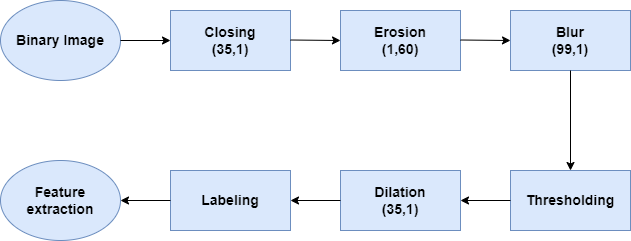
\includegraphics[width=11cm]{images/Flowchart_MO.png}
    \caption{Flowchart of the proposed method to extract contrast features for text line detection}
    \label{fig:Flowchart_MO}
\end{figure} 


\subsubsection{Finding Contours}

After the completion of the first stage, the next stage is to extract individual text lines present in the image. In order to extract individual text lines, a technique based on finding contours is used.\\

Contours are typically used to find a white object from a black background. All the above morphological operations are applied so that the Contours can detect the boundary edges of the blocks of text of the image.\\

Now, we can find all contours in the dilated image, check all the areas of each of the contours to identify which contours represent the text line and draw these contours to show all text lines in the image as shown in this figure \ref{fig:drawing}.

We can crop all these contours to extract individual text lines from an image as shown in this figure \ref{fig:crop}.

\begin{figure}[!htb]
     \centering
     \begin{subfigure}[b]{0.4\textwidth}
        \centering
        \includegraphics[width=6cm, height=9cm]{images/22_imgContoure1.png}
        \caption{After drawing contours.} 
        \label{fig:drawing}
     \end{subfigure}
     \hfill
     \begin{subfigure}[b]{0.4\textwidth}
        \centering
        \includegraphics[width=6cm, height=9cm]{images/lines_text.drawio.png}
        \caption{After cropping.} 
        \label{fig:crop}
     \end{subfigure}
    \caption{The sample after drawing contours and cropping}
    \label{fig:drawing-contours-cropping}
\end{figure}


\section{Word Segmentation}
the process of dividing the written text into meaningful units, such as words, and determining the word boundaries in a sentence or a document by computer algorithms.

\subsection{Functional Description}
 The cursive nature of the Arabic script such as the existence of different shapes for each character according to its location in the world besides the existence of diacritics makes Arabic character segmentation a very challenging task. A robust character segmentation algorithm for printed Arabic text with diacritics is developed based on the contour extraction technique. The algorithm works by extracting the up-contour part of a word and then identifies the splitting areas of the word characters. 

\subsection{Modular Decomposition}

\begin{itemize}[labelindent=1em,labelsep=0.25cm,leftmargin=*]

     \item[\char `A)] \textbf{Gray Scaling:- } \\ 
        This step to change the pixels of an image to gray in order to  make the image easier to analyze.
        applying grayscaling on the input line shown
        in figure\ref{fig:origin}  to grayscale shown in figure\ref{fig:gray}
        
        \item[\char `B)] \textbf{Thresholding:- } \\ 
        This step to change the pixels of an image to black and white in order to  make the image easier to analyze.
        applying thresholding on the grayscaled line shown in figure \ref{fig:thresh}
        
         \begin{figure}[H]
        \centering
        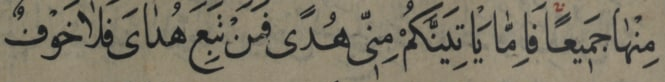
\includegraphics[width=10cm]{images/origin.png}
        \caption{Original Line}
        \label{fig:origin}
        \end{figure}
        
         \begin{figure}[H]
        \centering
        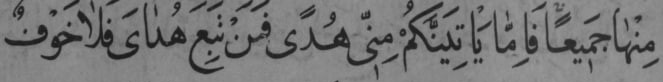
\includegraphics[width=10cm]{images/gray.png}
        \caption{Line after grayscaling}
        \label{fig:gray}
        \end{figure}
        
        \begin{figure}[!htb]
        \centering
        
\includegraphics[width=10cm]{images/threshoding.png}
        \caption{Line after thresholding}
        \label{fig:thresh}
        \end{figure} 
        \item[\char `C)] \textbf{Removing Dots:-}\\
        We applied to remove dots and Tashkel ,which have a very small area, in order to get the text itself to be easier to find each word as a separated contour.shown in figure \ref{fig:redots}
        \begin{figure}[!htb]
        \centering
        
\includegraphics[width=10cm]{images/removedots.png}
        \caption{Line after removing dots}
        \label{fig:redots}
        \end{figure} 
        \item[\char `D)] \textbf{Finding Contour:-}\\  
         In contour tracing \cite {contour} methods the pixels that form the outer shape of the character or word are extracted. Researchers used many ways to determine the cutting points on the contour. In general, contour-based methods avoid the problems that appear when applying thinning methods because they depend on extracting the structure of the word, which gives a clear description of it. This kind of method is sensitive to noise, which requires one to perform some enhancements as a pre-processing step.\\
         \newline
         Contour-based segmentation technique gives a clear description of the word characters shape. This method facilitates determining the right segmentation points.\\
         \newline
         Many methods have been tested to extract the contour of the abstracted word/sub-word image. The best results can be obtained when using the contour extraction method implemented into the \textbf{OpenCV} library named as \textbf{cv2.findContours()} function.
         \item[\char `E)] \textbf{Extracting Contoured Sub-words:-}\\
         After applying \textbf{cv2.findContours()} function,
         \textbf{cv2.drawContours()} from \textbf{Opencv} image processing toolbox used to draw a contour plot of the  image shown in figure \ref{fig:con2}. 
         and plotting each crop of each sub-word is visualized 
         by \textbf{cv2.drawContours()} shown in figure \ref{fig:con4}
         after cropping each sub-word is shown in figure \ref{fig:crops}.
    \end{itemize}
    
\begin{figure}[!htb]
    \centering
    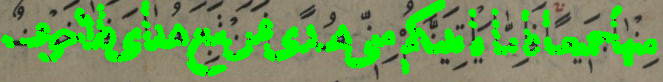
\includegraphics[width=10cm]{images/con2.png}
    \caption{Drawing Contours on each sub-word in the line}
    \label{fig:con2}
\end{figure} 

\begin{figure}[!htb]
    \centering
    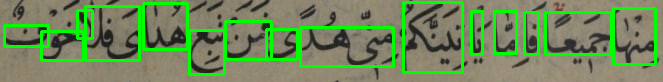
\includegraphics[width=10cm]{images/con4.png}
    \caption{Drawing Rectangle on each sub-word in the line}
    \label{fig:con4}
\end{figure} 

\begin{figure}[!htb]
    \centering
    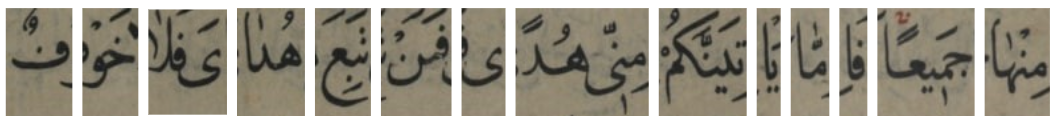
\includegraphics[width=10cm]{images/crops.png}
    \caption{Cropping each sub-word from the line}
    \label{fig:crops}
\end{figure} 

\clearpage

\section{Word Spotting}
This module is responsible for applying word spotting methods, that's because of the huge variability and noise in historical handwritten documents it is inaccurate to use OCR techniques to extract information. This project focuses on word spotting techniques with Deep learning in order to digitize information in handwritten documents and accelerate historic research.

\subsection{Functional Description}
In this module, we will apply different techniques for word spotting and recognition to achieve the best recognition accuracy in different conditions. \\

Since the goal in word spotting is to retrieve parts of document images that are relevant with respect to a certain user-defined query, and in order to get a better recognition accuracy. We used \acrshort{phosc} algorithm which is a hybrid technique from \acrshort{phoc} and \acrshort{phos} algorithms which will be explained in detail in the following subsections. 

\subsection{Modular Decomposition}
This module could be separated into a number of distinct sub-modules depending on each other. 

\subsubsection{PHOC} 
In order to understand the text and image content, word spotting and word recognition are suitable approaches. It sounds very similar to each other but is two different tasks.
\begin{itemize}[itemsep=1pt, topsep=5pt]
    \item \textbf{Word Spotting}. \\
    Given an image containing a word as input, word spotting refers to detecting other image segments in the document exhibiting patterns similar to the query image. \\
    The goal is to find all instances of a query word in a dataset of images. The query word may be a text string in which case it is usually referred to as \acrfull{qbs}. Or maybe also an image, in which case it is usually referred to \acrfull{qbe} \cite{WORDSPOTTING}. \\
    
    In \acrshort{qbs} word is represented in text form for retrieval, and is converted to equivalent image representation before searching inside the document. While in \acrshort{qbe} example word image is provided for retrieving relevant matches inside the document. The example word image is also called \emph{template matching} which is based on the visual similarity of the test word images.
    
    \item \textbf{Word Recognition} \\
    Given an image containing a word as input, the word recognition system identifies the word from the lexicon that is present in the image. \\
    The goal is to obtain a transcription of the query word image, figure \ref{fig:wordspotting-vs-wordrecognition} shows the differences.
    \begin{figure}[!htb]
        \centering
        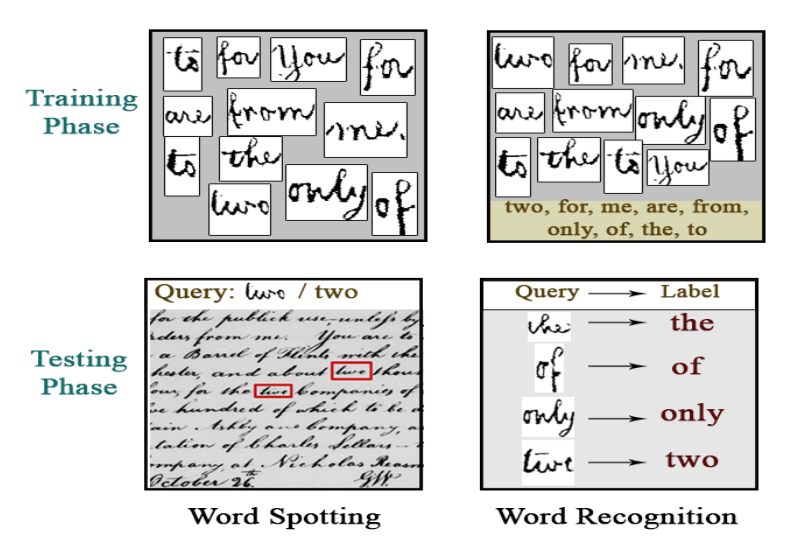
\includegraphics[width=11cm]{images/wordspotting-vs-wordrecognition.png}
        \caption{Difference between word spotting and recognition}
        \label{fig:wordspotting-vs-wordrecognition}
    \end{figure}
\end{itemize}

\noindent
Since word spotting and word recognition are important tasks for digitizing manuscripts documents, a common representation for word images and text strings is introduced. Using this representation, spotting and recognition become simple nearest neighbor problems. A label embedding approach for text labels inspired by the bag of characters string kernels used for example in machine learning. This approach embeds text into a $d$ dimensional binary space called \acrfull{phoc}, which encodes if a particular character appears in a particular spatial region of the string (shown in \ref{fig:phoc_histogram}), then this embedding is used as a source of character attributes, and in addition to each word image will be projected into another dimensional space. Then, each dimension encodes how likely that word image contains a particular character in a particular region, in obvious parallelism with the PHOC descriptor. By learning character attributes independently, training data is better used and out of vocabulary (OOV) spotting and recognition is straightforward. \\

\noindent
The goal of the combination of word spotting and word recognition is to find a common subspace between attributes and PHOCs. Learning the common subspace from training data that has images and corresponding text strings is shown in figure \ref{fig:phoc_common_subspace}. \\

\begin{figure}[!htb]
    \centering
    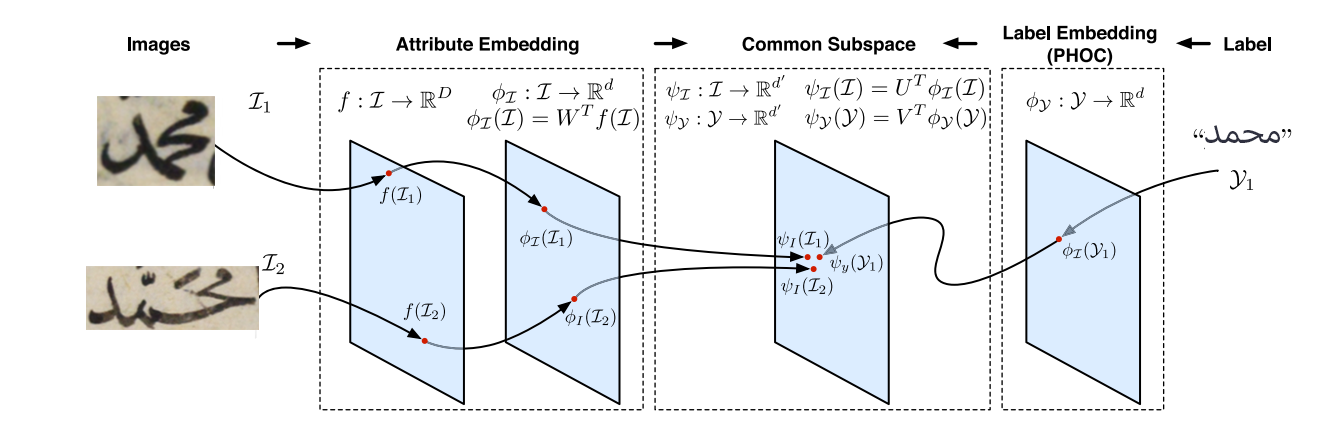
\includegraphics[width=15cm]{images/phoc-common-subspace.png}
    \caption{PHOC training process}
    \label{fig:phoc_common_subspace}
\end{figure}

Since PHOC embeds the text string to construct a (binary) histogram of characters, some words like "\<كلمات>" and "\<تكامل>" will have the same representations. Therefore, PHOC focus on different regions of the word at different levels as shown in figure \ref{fig:phoc_histogram}. The 4 levels are used to construct PHOC dimensions which each level will split the word into specific parts (for example level 2 will split the word into 2 parts, level 3 into 3 parts, and so on). Then, finally, PHOC representation will be the concatenation of these histograms. So the PHOC dimensions will be (2+3+4) $x$ 45 = 405 dimensions. In addition, we also add the most common Arabic bigrams at level 2, leading to 100 extra dimensions for a total of 505 dimensions. These bigrams let us encode relations between adjacent characters, which may help to disambiguate when finding a low-dimensional common subspace.

\begin{figure}[!htb]
    \centering
    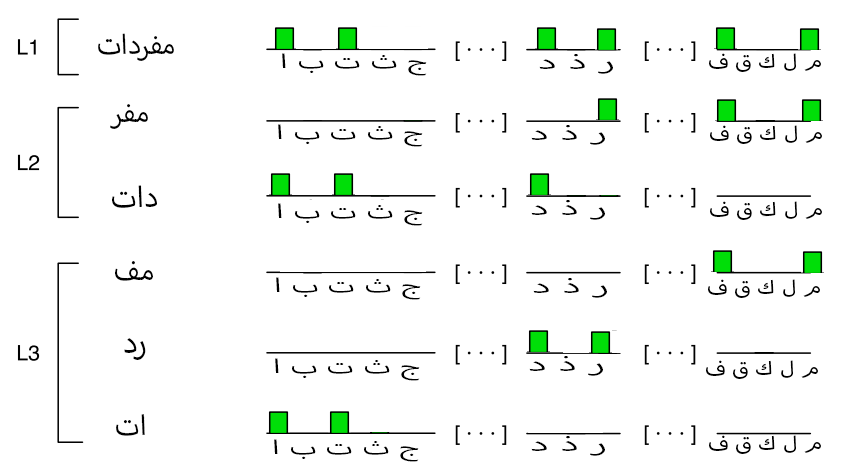
\includegraphics[width=10cm]{images/phoc_representation-arabic.png}
    \caption{PHOC histogram of a word at levels 1,2, and 3}
    \label{fig:phoc_histogram}
\end{figure}

\acrfull{cnn} has an effective role when dealing with images and found its way to analyze document images \cite{PHOCNET}. So PHOCNet is a CNN architecture specifically designed for word spotting and by using \acrshort{phoc} as labels, This CNN is able to achieve the state-of-the-art performance in \acrfull{qbe} as well as \acrfull{qbs} scenarios.\\

CNN architectures can generally be split into two parts. The first is the convolutional part which usually constitutes convolutional and pooling layers. Convolutional layers consist of a number of so called \emph{filters} with which the input image is convolved. The output is a number of feature maps that can be the input to another layer of the CNN. Each feature map is produced by applying one of the filters in the respective convolution layer to the input. In order to introduce non-linearity into CNNs, the output of convolutional layers is passed through an activation function. Traditionally, the activation function of choice has been the sigmoid function in the following equation.
\begin{equation}
    sg(x) = \frac{1}{1 + e^-x}
    \label{equ:sigmoid}
\end{equation}

After applying the activation function the receptive field size can be expanded by using Pooling layers. These CNN layers aggregate filter responses by down-sampling the feature map. The predominant pooling strategy in deep CNNs has been Max Pooling. In Max Pooling, the filter responses over a certain local region are taken and only the maximum filter response is passed
to the next layer. \\
The convolutional part of a CNN can be thought of as producing a feature representation that can be fitted to the data at hand in a supervised manner. After this part, deep CNNs usually make use of a standard \acrfull{mlp} as a classifier. Here, multiple so called fully connected layers are stacked together to form the MLP. In usual single label image classification tasks, training a CNN is carried out by first applying the softmax function

\begin{equation}
    sm(o)_i = \frac{e^o_i}{\sum_{j=1}^n e^o_j} = \hat y_i
\end{equation}

The output $o$ of the last layer of the CNN in order to generate
the output vector $\hat y$ of predicted pseudo class probabilities. This can be seen as adding a special non-linear scaling layer to the CNN. In order to adapt the parameters to the data, the cross entropy loss $l$ between the one-hot encoded label vector y and $\hat y$ is computed as The error is then backpropagated through the network \\

\noindent
The general architecture of PHOCNet is visualized in figure \ref{fig:phocnet}. The design is consist of 3x3 convolutions followed by \acrfull{relu} in the convolutional parts of the neural network. Usually, CNNs are fed with images of the same width and height. Most word images would thus have to be either cropped or rescaled. So we resized the images with 70x90 pixels resolution. After convolutional and max pooling layers, there is a special pooling layer called Spatial Pyramid Pooling. This type of layer allows CNNs to accept different sized input images and still produce a constant output size which is essential for training the network. 3-level Spatial Pyramid max pooling to circumvent the need for cropping or resizing the input image. \\

In order to train a deep CNN with PHOCs, the softmax layer can no longer be used as only one element in the training vector is 1 whereas multiple elements of the PHOC label can be 1. However, training the CNN with PHOCs as labels can be seen as a multi-label classification task. Thus, the softmax function is used instead of sigmoid activation function. This way, each attribute is interpreted as a label in a multi-label classification task with cross entropy loss in equation\ref{equ:phoc-loss}.

\begin{equation}
    l(y,\hat y) = - \frac{1}{n} \sum_{i=1}^n [y_i \: log \hat \: y_i + (1 -y_i)\, log(1-\hat y_i)]
    \label{equ:phoc-loss}
\end{equation}

\begin{figure}[!htb]
    \centering
    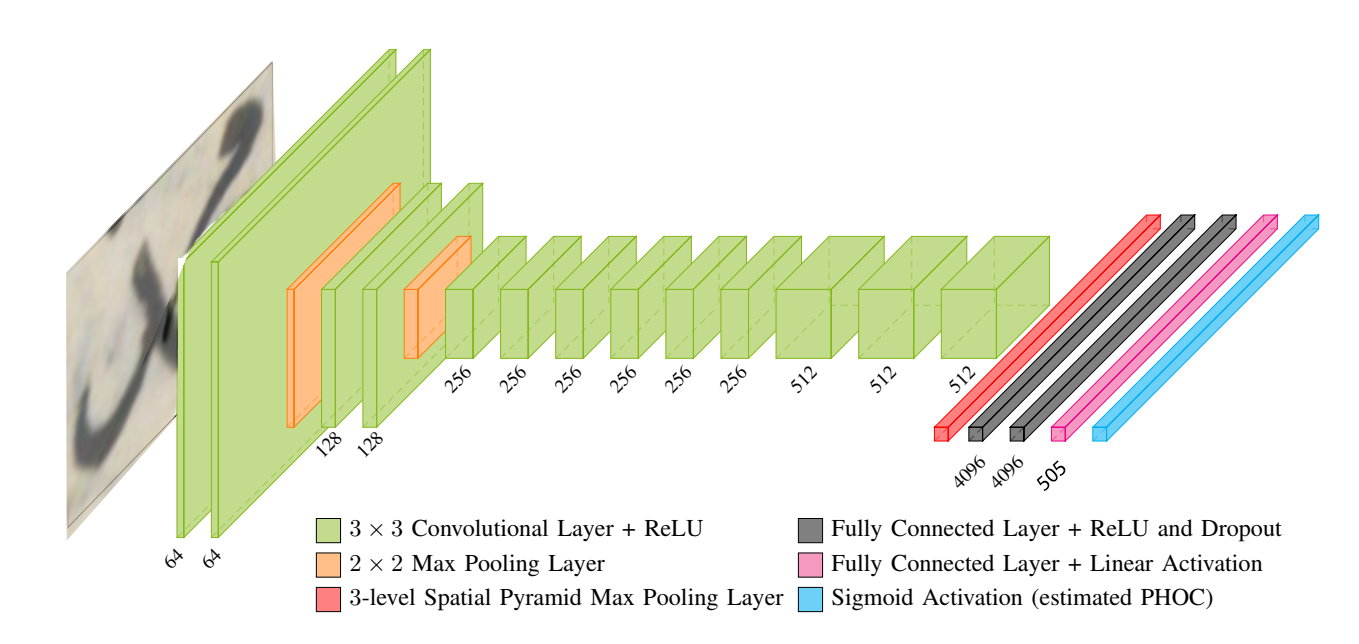
\includegraphics[width=16cm]{images/phocnet.PNG}
    \caption{PHOCNet Architecture}
    \label{fig:phocnet}
\end{figure}

\subsubsection{Zero Shot Learning}
In the previous section, we did explain PHOCNet which applies PHOC representation method in both word spotting and recognition. Word recognition based systems require enough labeled data per class to train the system. Moreover, all word classes need to be taught beforehand. Though word spotting could evade this drawback of prior training, these systems often need to have additional overheads like a language model to deal with \acrfull{oov} words. Zero-shot learning could be a possible alternative to counter such a situation. \\

Zero-shot Learning is a relatively new branch of Machine Learning which is useful when there is no assurance of sufficient annotations for all possible classes and objects to be classified. One must take into account that annotations/class labels for some classes are easy to obtain in comparison to other classes in any image classification problem. This is due to scarcely available images for labeling which can only be made by a human expert in a particular domain. Then, Zero-shot learning algorithm is capable of handling unseen classes, provided the algorithm has been fortified with rich discriminating features and reliable \textbf{attribute description} per class during training. \\

In the context of Zero-shot learning “class/attribute signatures”, represent semantic information about classes involved in the training and testing of the system. A “class/attribute signatures” represents some unique visual/semantic characteristics of the associated class which clearly makes a distinct mark of the difference from other classes involved in the classification process. For example, to recognize/classify/differentiate between a cat and other wild carnivorous animals, the presence of black stripes on the body of the cat could be used as one of the most obvious “class/attribute signature”. The value for this “class/attribute signature” could be set to 1 for the “Cat class” and 0 for other classes. Since images of Text/Words are devoid of such glaring visual clues, we need to rely on the presence of primitive shape structures in the shape of the word, to procure different “class/attribute signature” values. These word class attribute signatures do take into account character order in a general way, but at the cost of longer vector dimensions \cite{ZEROSHOT}.

\subsubsection{PHOS}
In \acrfull{zsl}, the test query images can contain words that the model did not see during training. This is a more challenging task requiring a visual representation (akin to the semantic embedding in \acrshort{zsl} literature) that can bridge the set of seen and unseen words. A visual characterization of words to learn a mapping between word-images and their corresponding word labels such that it can also be used to recognize out-of-lexicon words called \acrfull{phos} \cite{PHOSC}. The PHOS representation encodes the primary shapes of character strokes of different word segments in a hierarchical manner. We use a deep convolutional network to learn the PHOS representation from images of words present in the training lexicon. \\

Since \acrshort{phos} encodes the visual features of the characters (perform zero-shot word recognition) that are missed by PHOC and therefore is more suitable to recognize unseen words. Central to the PHOS representation is the assumption that every character can be described in terms of a set of primitive shape attributes \cite{ZEROSHOT}. We consider the following set of primitive shapes for Arabic language as illustrated in figure\ref{fig:arabic-primary-shape}. Only the counts of these shapes is insufficient to adequately characterize each word uniquely. Inspired by the pyramidal capture of occurrence and position of characters in a word, we propose the pyramidal histogram of shapes that helps in characterizing each word uniquely.

\begin{figure}[!htb]
    \centering
    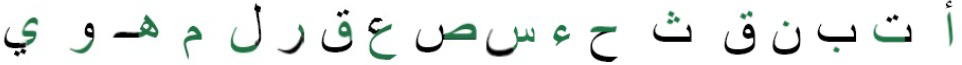
\includegraphics[width=14cm]{images/arabic-letters.png}
    \caption{18 primary shape attributes}
    \label{fig:arabic-primary-shape}
\end{figure}


The process of capturing the PHOS representation for a word is illustrated in figure \ref{fig:phos-representation}. At the highest level of the pyramid, there exists only a single segment, which is the entire word. At every level h of the pyramid, we divide the word into h equal segments. Further, at every level h, we count the occurrence of the 18 primary shapes in every h segment of the word. The concatenation of the count vectors for every segment in a level and across all the levels of the pyramid results in the PHOS representation of the word. In this work, we have used levels 1 through 5, resulting in a PHOS vector of length (1+2+3+4)*18 = 180. Thus the PHOS vector encodes the occurrence and relative position of the shapes in the word string.

\begin{figure}[!htb]
    \centering
    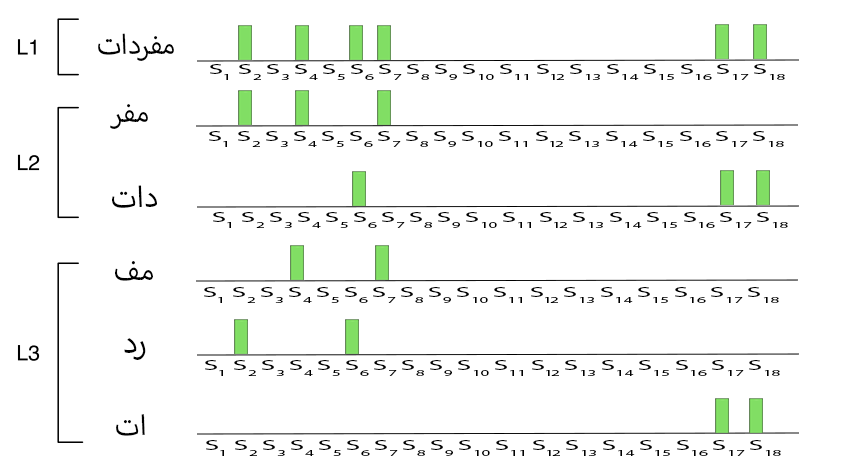
\includegraphics[width=10cm]{images/phos_representation-arabic.png}
    \caption{Pyramidal structure of PHOS representation}
    \label{fig:phos-representation}
\end{figure}

\subsubsection{PHOSC}
For the zero-shot word recognition problem, it is important to encode the occurrence and relative position of characters within a word, as well as that of visual shapes. Therefore, a new method is proposed to use the concatenated PHOC and PHOS vector of a word as its attribute signature representation $C$. Thus, the attribute signature representation for the word label $y_i$ is $[c_c(y_i), c_s(y_i)]$ where $c_c(y_i)$ and $c_s(y_i)$ are the PHOC and PHOS representations respectively. \\

\acrfull{phosc} is a multi-task network with shared feature extraction layers between the two tasks (PHOC and PHOS). The shared feature extraction network is a series of convolution layers, followed by a spatial pyramid pooling (SPP) layer. The SPP layer facilitates the extraction of features across multiple image resolutions. PHOSC separates out into two branches after the SPP layer to output the two representations. The two branches contain two independent fully connected layers. As the PHOC representation is a binary vector, the PHOC branch ends with a sigmoid activation layer. On the other hand, the PHOS representation being a non-negative vector, the PHOS branch ends with a ReLU activation layer. The multi-task Pho(SC)Net architecture is illustrated in figure \ref{fig:phosc-arachitecture}.

\begin{figure}[!htb]
    \centering
    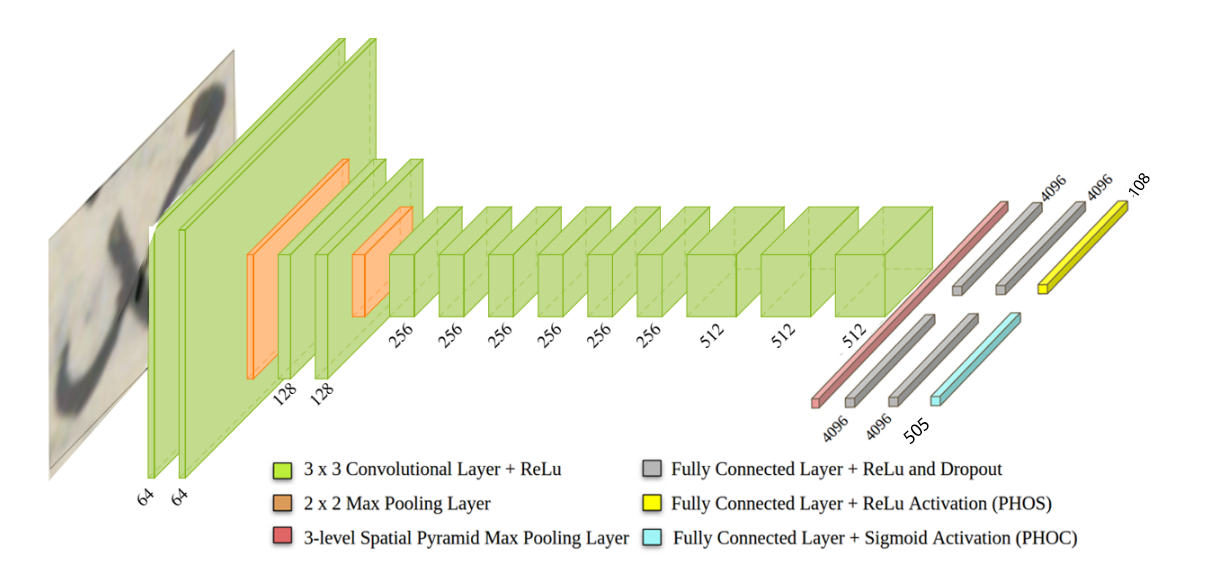
\includegraphics[width=16cm]{images/phosc-archiecture.png}
    \caption{Architecture of PHOSCNet}
    \label{fig:phosc-arachitecture}
\end{figure}

The output of the PHOSCNet for an input word image is the vector $\phi(x) = [\phi_C(x), \phi_S(x)]$ where $\phi_C(x)$ and $\phi_S(x)$ are the predicted PHOC and PHOS representations respectively. Given a mini batch of B instances from the training set consisting of seen word images and their labels, we minimize the following loss function during training.

\begin{equation}
    L= \sum_{i=1}^B \lambda_c L_c(\phi_c(x_i), c_c(y_i)) + \lambda_s L_s(\phi_s(x_i), c_s(y_i))
    \label{equ:phosc-loss-function}
\end{equation}

Where $L_c(phi_c(x_i), c_c(y_i))$ is the cross entropy loss between the predicated and actual PHOC representations, $L_s(phi_s(x_i), c_s(y_i))$ is the squared loss between the predicated and actual PHOS representations, and $\lambda_c , \lambda_s$ are hyper-parameters used to balance the contribution of the two loss functions. \\

Given a test image $x$, the PHOSCNet is used to predict the PHOC and PHOS representations to obtain the predicted attribute signature representation $[\phi_c(x), \phi_s(x)]$. The  word whose attribute signature representation has the highest similarity (measured as cosine similarity) is the predicted word label for the test image, in the conventional ZSL, as defined below
\begin{equation}
    \hat y = argmax_{k\in y^u} \: cos([\phi_c(x), \phi_s(x)]^T[c_c(k), c_s(k)])
    \label{equ:cosine-similarity}
\end{equation}

\section{Model Development}
This module is responsible for developing the model to be ready for predicting unseen words with different styling. This module will include model development stages like data preparing, data augmentation, and training hyperparameters.

\subsection{Functional Description}
This module takes the segmented words image from the page segmentation module and embedded it into the model after being trained on a lot of labeled data which will be introduced in the following subsections.


\subsection{Modular Decomposition}
Our model consists of two main models: training data, and network hyperparameters, like any deep learning model. Training data is the preprocessing steps to be done on the image data, in order to prepare it for network training. Network hyperparameters are in which you determine the network settings to fit the training data and for better understanding of our task, in order to better prediction in real world and unseen data.

\subsubsection{Data Preparing and Cleaning}

We have mentioned in the survey stage that we studied more than one dataset and got acquainted with the advantages and disadvantages of each dataset of them, as well as the extent to which each dataset of them agrees with the idea that we want to implement and also with the method of work that we agreed to work on during the project and the dataset was the most suitable for our conditions and the readiest To work and most compatible with the method of work that we decided to work with is the VML-HD dataset that was created by a group of researchers at a university and they made a great effort to prepare it and made it available to everyone. This is a thankful position for them on the scientific level. this dataset consists of images and an attached xml file in HADARA format generated by the WEB-GT website.

The stage of exploring the dataset and preparing it for work was a very difficult stage, and we faced many problems that we had to deal with professionally in order to ensure good performance during the work.
This stage has been divided into sub-stages as follows:
\begin{itemize}
  \itemsep0em
  \item Dataset Loading
  \item Data Understanding
  \item Dataset Exploration
  \item Data Cleaning
\end{itemize}

\paragraph{Dataset Loading}\mbox{}\\
Here the VML-HD dataset has been downloaded from its official website and on the website, there are two versions of the dataset, the first is the dataset is complete images of the pages of the manuscripts that have been selected to work in this dataset and the second is the dataset after it has been hashed into subwords and we had to This situation determines which of the two versions we will choose to work, the two versions and their studies have been uploaded to determine the best and most appropriate from our point of view.
After downloading the data files from the internet, we will do the data cropping process using the image files and the XML file attached to the data, which we have already mentioned is created from the WEB-GT framework.

\paragraph{Data Understanding}\mbox{}\\
After downloading the dataset, we began to study it in-depth, get to know it closely, understand it, find its strengths and weaknesses, and also choose which of the two versions on the official website is the best for us and the most suitable for work.
And I found the data set in general based on five books written by different writers in the years 1088 - 1451, The five books that were exported for the work were named as follows: 3157556, 3158466, 3249138, 3368132, and 3426930. The 668 pages are fully annotated on the subword level. For each page, the team that created this dataset manually applied bounding boxes on the different subwords and annotated the sequence of characters. It consists of 159,149 sub-word appearances consisting of 326,289 characters out of a vocabulary of 5,509 forms of sub-words.
This information is the information on the website about the dataset and will be subject to study and validation at the stage of dataset exploration.

\paragraph{Dataset Exploration}\mbox{}\\
Data exploration refers to the initial step in data analysis in which data analysts use data visualization and statistical techniques to describe descriptions of a data set, such as size, quantity, and accuracy, in order to better understand the nature of the data.
In the exploration phase, we studied the dataset in a deep study, the aim of which is to identify the data more clearly and also to know the nature of the dataset closely, determine its strengths and weaknesses, and apply some descriptive and inferential statistical rules to it as much as possible.
We mentioned that the five books that were exported for work were named as follows: 3157556, 3158466, 3249138, 3368132, and 3426930, and here we will review some statistical results for each of them in the table\ref{table:statistics_for_each_book}.

\begin{table}[!htb]
\centering
\begin{tabular}{|l|c|c|c|c|c|}
\hline
STATISTICS OF THE BOOK & 3249138 & 3157556 & 3158466 & 3426930 & 3368132 \\  \hline
Number of pages & 101 & 196 & 136 & 136 & 94 \\ \hline 
Number of lines &  1414  & 1656 & 2022 & 1596 & 1860 \\ \hline 
Number of words & 27274  & 28671 & 34791 & 31697 & 35456 \\ \hline 
Number of classes & 2539 & 2471 & 2751 & 3200 & 1770 \\  \hline 
Average number of words per page & 270.04 & 146.28 & 255.82 & 226.41 & 377.19 \\ \hline 
Average number of lines per page & 14.0 & 8.45 & 14.87 & 11.4 & 19.79 \\ \hline
Average number of words per line & 19.29 & 17.31 & 17.21 & 19.86 & 19.06 \\\hline
Average number of words classes & 10.74 & 11.6 & 12.65 & 9.91 & 20.03\\  \hline
\end{tabular}
\caption{The statistics for each book.}
\label{table:statistics_for_each_book}
\end{table}

\noindent
In general, at the level of the whole data set, we find that we have reached these descriptive statistics, which are shown in a table\ref{table:statistics_for_all_dataset}

\begin{table}[!htb]
\centering
\begin{tabular}{|l|c|}
\hline
Total number of pages & 668 \\ \hline
Total number of lines & 8548 \\ \hline
Total number of words & 157889 \\ \hline
Total number of classes & 6180 \\ \hline
\end{tabular}
\caption{Total statistics of the books.}
\label{table:statistics_for_all_dataset}
\end{table}

\newpage

\paragraph{Data Cleaning}\mbox{}\\
Data cleaning is the process of repairing or removing invalid, damaged, incorrectly formatted, duplicate, or incomplete data within a data set. When merging multiple data sources, there are many opportunities for data to be duplicated or misnamed. If the data is incorrect, the results and algorithms are unreliable, even though they may appear correct. There is no one absolute way to describe the exact steps in the data cleaning process because the processes will vary from dataset to dataset. But it's important to design your data cleaning process so you know you're doing it the right way every time.
After the process of data cropping based on the XML file, we found that there are some classes that do not fit the work and have errors, such as the classes called by names "k", "mislabel" , \<ءية> , \<ءء> , \<ءه> etc...\\


Since the people who created this dataset and gave it names are not Arabs and do not know the Arabic language well, there were many categories that they had named wrongly and some of the similar letters between them did not differentiate between them during the names such as letters \<حـ>, \<جـ>, \<غ>, \<ع>, \<ز> , \<ر> and other.
As well as changing some letters in one word, such as \<نلعنهم> they know it with \<نعلنهم> and \<يمنيهم> know it with \<يمينهم> and other.

\paragraph{Data Augmentation}\mbox{}\\

\noindent
The quantity and variety of data are important factors in the effectiveness of most machine learning models. The quantity and diversity of data provided during training greatly influence the prediction accuracy of these models.
Applying a set of transformations to the available data to collect new data is one technique for dealing with the challenge of limited data. Data augmentation refers to the process of collecting new data from existing data.\\

Data augmentation is a set of techniques used to increase the amount of data in a machine learning model by adding slightly modified copies of already existing data or newly created synthetic data from existing data. Helps streamline the machine learning model and reduce data overprocessing.
we use the homography Augmentation method to increase data, this creates an augmentation by computing a homography from three points in the image to three randomly generated points.
Then we used Affine Transformation from the OpenCV library, A transformation that can be expressed in the form of matrix multiplication (linear transformation) followed by a vector addition (translation).

\noindent
An example of data augmentation shown in the figure \ref{fig:Data Augmentation Example}

\begin{figure}[!htb]
     \centering
     \begin{subfigure}[b]{0.2\textwidth}
         \centering
         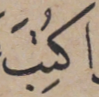
\includegraphics[width=2cm, height=2cm]{images/original.png}
         \caption{Original image}
         \label{fig:Original image}
     \end{subfigure}
     \hfill
     \begin{subfigure}[b]{0.8\textwidth}
         \centering
            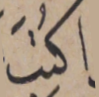
\includegraphics[width=2cm, height=2cm]{images/augmented_0.png}
            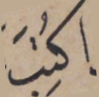
\includegraphics[width=2cm, height=2cm]{images/augmented_1.png}
            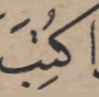
\includegraphics[width=2cm, height=2cm]{images/augmented_2.png}
            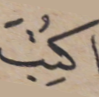
\includegraphics[width=2cm, height=2cm]{images/augmented_3.png}
            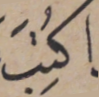
\includegraphics[width=2cm, height=2cm]{images/augmented_5.png}
            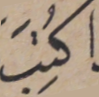
\includegraphics[width=2cm, height=2cm]{images/augmented_6.png}
         \caption{Sample of augmented images }
         \label{fig:Sample of augmented images}
     \end{subfigure}
        \caption{Data Augmentation Example}
        \label{fig:Data Augmentation Example}
\end{figure}

\newpage
\subsubsection{Model Hyperparameters} 
Hyperparameter tuning is an essential part of controlling the behavior of the  model. If we don’t correctly tune our hyperparameters, our estimated model parameters produce sub optimal results, as they don’t minimize the loss function. \\

Hyperparameter tuning consists of finding a set of optimal hyperparameter values for a learning algorithm while applying this optimized algorithm to any data set. That combination of hyperparameters maximizes the model’s performance, minimizing a predefined loss function to produce better results with fewer errors.\\

\noindent
Here is a list of hyperparamaters that we used in our model :
\begin{itemize}[itemsep=1pt, topsep=5pt]
    \item \textbf{Number of Hidden layers:-}\\
    Different layers can affect the accuracy like fewer layers may give an underfitting result while too many layers may make it overfitting. So, our model consists of:
    \begin{itemize}[itemsep=1pt, topsep=5pt]
    \item Input layer which takes the input shape of the image 
    \item 2 Conv2D layers with 64 filter of size (3*3),padding='same' and  activation='relu' 
    \item 1 MaxPooling2D with kernal of size (2*2) and stride=2 
    \item 2 Conv2D layers with 128 filter of size (3*3),padding='same' and  activation='relu' 
    \item 1 MaxPooling2D with kernal of size (2*2) and stride=2
    \item 6 Conv2D layers with 256 filter of size (3*3),padding='same' and  activation='relu' 
    \item 3 Conv2D layers with 512 filter of size (3*3),padding='same' and  activation='relu'
    \item SpatialPyramidPooling2D layer, preforms pooling using three different pooling layers [1,2,4]  
    \item Flatten layer, to convert matrix to vector 
    \item 2 Dense layer with 4096 neurons, activation='relu' and Dropout=0.5
    \item Dense layer with 180 neurons, activation='relu' for PHOS model
    \item 2 Dense layer with 4096 neurons, activation='relu' and Dropout=0.5  
    \item Dense layer with 505 neurons, activation='sigmoid' for PHOC model
    \item Output layer (PHOSC) which is hybrid  from PHOS model and PHOC model.
\end{itemize} 
    \item \textbf{Number of Neurons per Layer:-}\\
    The number of neurons in every layer is set to be the same. It also can be made different. The number of neurons should be adjusted to the solution complexity. The task with a more complex level to predict needs more neurons.\\
    the structure of the model shown in figure \ref{fig:layers}

    \item \textbf{Activation Function:-}\\
     An activation function is a parameter in each layer. Input data are fed to the input layer, followed by hidden layers, and the final output layer. The output layer contains the output value. The input values moving from a layer to another layer keep changing according to the activation function. The activation function decides how to compute the input values of a layer into output values. The output values of a layer are then passed to the next layer as input values again. The next layer then computes the values into output values for another layer again.\\
     We used:-
     \begin{itemize}[itemsep=1pt, topsep=5pt]
        \item Relu activation function:
        in the hidden layers and the output layer of PHOS model 
        \item Sigmoid activation function:
        in the output layer of PHOC model.  
     \end{itemize} 
     \item \textbf{Strides:-}\\
     We used strides=2 in the max pooling kernel, and for dimensionality reduction.
    
     \item \textbf{Dropout:-}\\
     We used  Dropout=0.5 in both PHOC and PHOS model,
      Dropout is used to regularize our model and reduce overfitting.
    \item \textbf{Losses:-}\\
     We used :
     \begin{itemize}[itemsep=1pt, topsep=5pt]
        \item Cross-Entropy Loss in PHOC model: cross-entropy arises as the natural cost function to use if a sigmoid  non-linearity in the output layer of the network, and maximizes the likelihood of classifying the input data correctly.
        \item Means Squared Error (MSE) in PHOS model: It is the right loss for regression, where the distance between two
values that can be predicted are small.
     \end{itemize} 
     \item \textbf{Optimizer:-}\\
     We used \textbf{Adam} optimizer with learning rate = 1e-4 and weight decay=5e-5.
     
    \item {\textbf{Callbacks}} \\
    We have two build-in Tensorflow callbacks
    \begin{itemize}[itemsep=1pt, topsep=5pt]
        \item Early Stopping: mainly used to avoid overfitting.
        \item ReduceLROnPlateau: mainly used to monitors a quantity and if no improvement is seen for number of epochs, the learning rate is reduced.
     \end{itemize} 
    
     \item {\textbf{Batch Size} = 32}
     \item {\textbf{Epochs} = 50}
     \item {\textbf{Learning rate} = 1e-4} \\
     learning rate controls the step size for a model to reach the minimum loss function. A higher learning rate makes the model learn faster, but it may miss the minimum loss function and only reach the surrounding of it. A lower learning rate gives a better chance to find a minimum loss function shown in figure \ref{fig:lr}. As a tradeoff lower learning rate needs higher epochs, or more time and memory capacity resources.
     
     \begin{figure}[!htb]
        \centering
        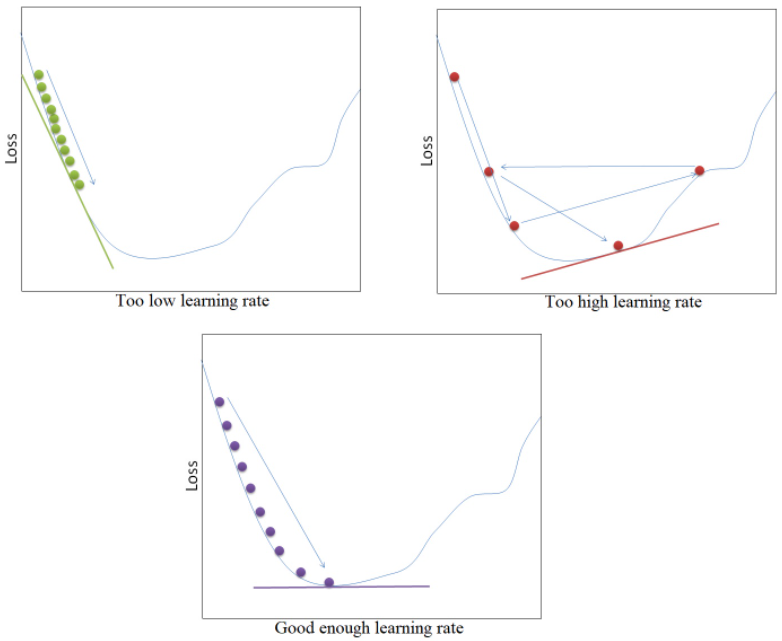
\includegraphics[width=6cm]{images/lr.png}
        \caption{Learning rate illustration.}
        \label{fig:lr}
    \end{figure}
    
    \begin{figure}
        \centering
        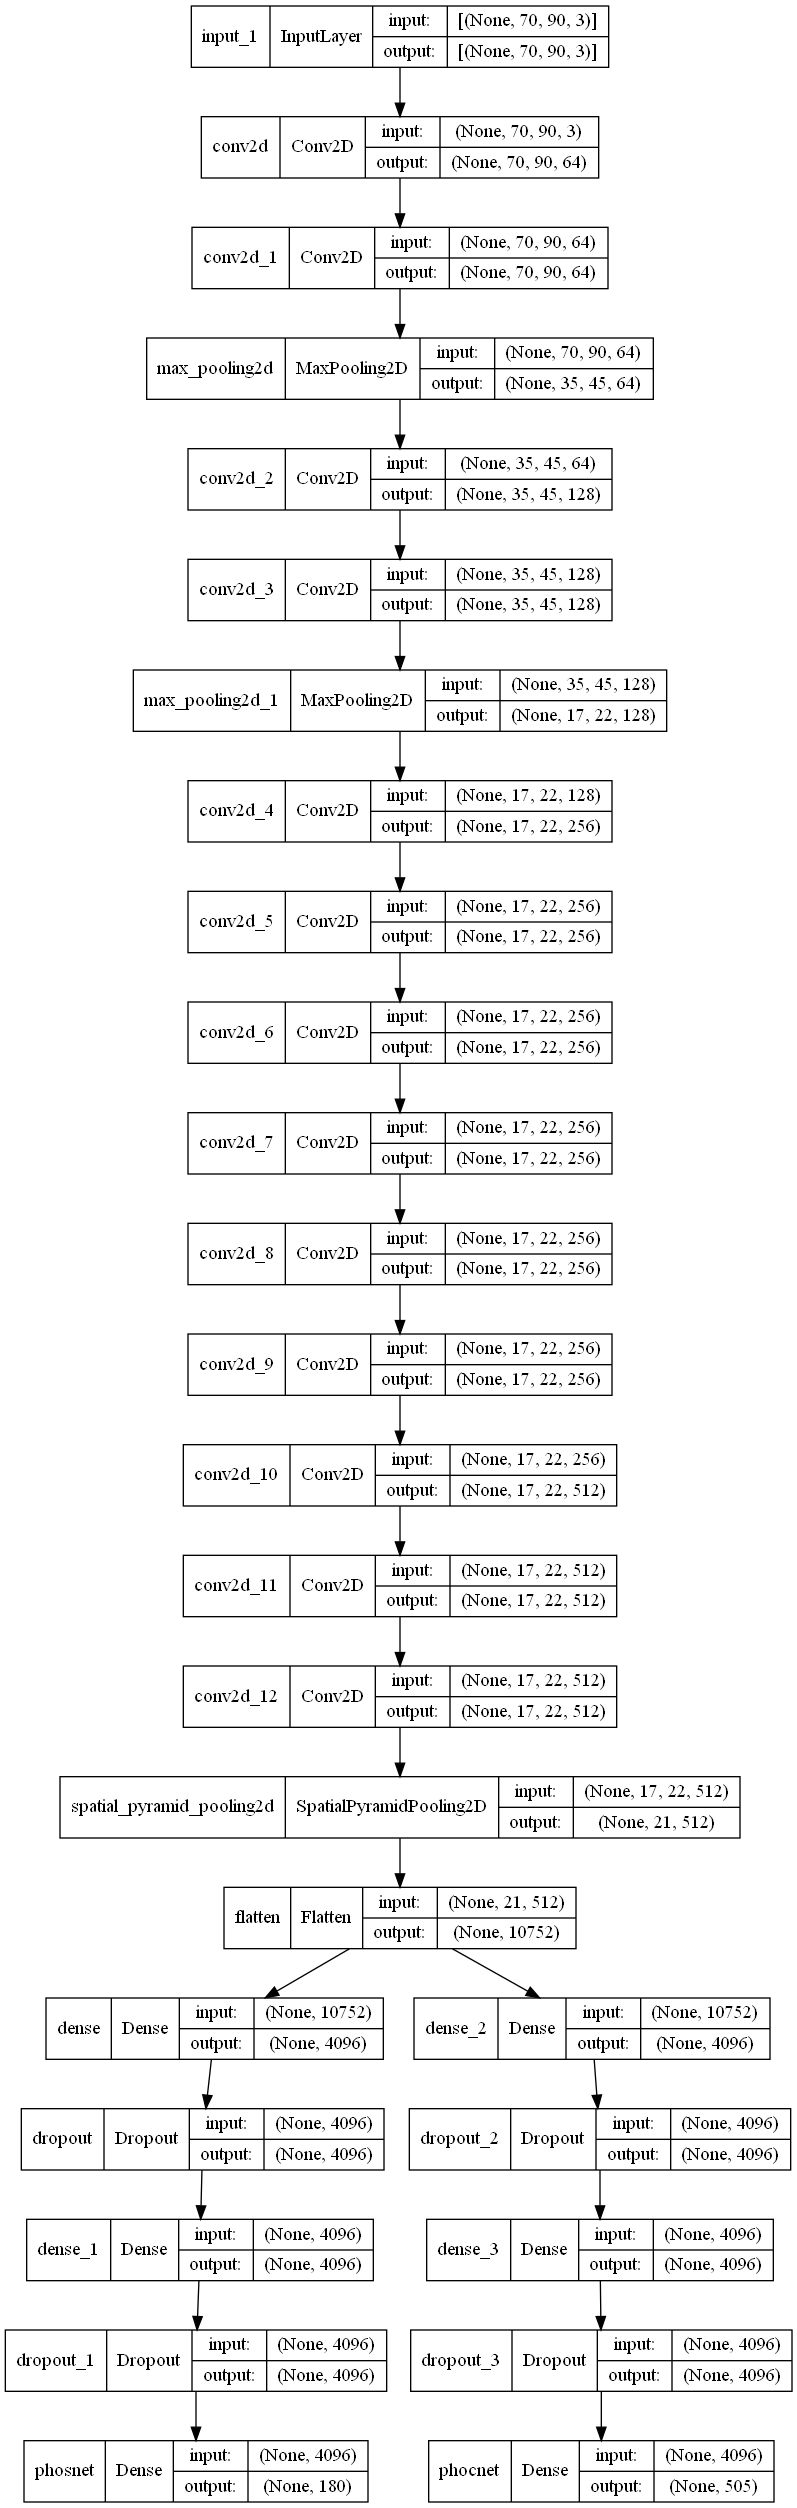
\includegraphics[width=10cm, height=23cm]{images/layers.png}
        \caption{The structure of PHOSC model.}
        \label{fig:layers}
    \end{figure}
    
\end{itemize}

